\documentclass[a4paper]{article}
\usepackage[english]{babel}
\usepackage[utf8]{inputenc}
\usepackage{amsmath}
\usepackage{graphicx}
\usepackage[colorinlistoftodos]{todonotes}
\usepackage{setspace}
\usepackage[margin=1.15in]{geometry}
\setlength{\parskip}{\baselineskip}
\setlength{\parindent}{0pt}

\title{QF603 Group Mini-Project 1}

\author{Group F}

\date{\today}

\begin{document}
	\maketitle
	
	\begin{abstract}
		In this report, we examined the S\&P500 and Dow Jones Industrial Average (``DJIA'') indices. Specifically, we studied the distribution of their returns as well as the correlation between those returns. The conclusion from our research is that the daily log returns of both the S\&P500 and the DJIA are not normally distributed. Also, we noted that although both indices are highly correlated in the long run, there are periods where the correlation weakens.
	\end{abstract} 
	
	\section{Task 1}
	\label{sec:introduction}
	
	\subsection{Verification of Dow Jones index}
	\setstretch{1.4}
	The value of the DJIA index per our calculations is 25,379.45, and the reported value of the index is also 25,379.45 (source: Bloomberg). There is a miniscule difference of $1.183\cdot10^5\%$ which can be considered a rounding error. Therefore, the closing price of the DJIA index reported by Bloomberg on the 18th of October 2018 is not different from the calculated value.
	
	
	\subsection{Findings about S\&P 500}
	The popular S\&P 500 (also known as ``S\&P'') , known in full as the Standard \& Poor’s 500, once took humbler forms. First called “The Composite Index”, the initial form of the S\&P tracked only a handful of stocks when Poor’s Publishing introduced it in 1923. The index saw its number of tracked stocks increase to 90 in 1926, and in 1941, Poor’s Publishing merged with Standard Statistics to form Standard \& Poor’s Corporation. It was only until 4 March 1957 that the index saw its number of tracked stocks increase to 500 and its name changed to the “S\&P 500” that we are all more familiar with. Only a handful of the S\&P’s original members, such as Coca-Cola, Pfizer and PepsiCo are still in the index today.
	
	Unlike the older Dow Jones Industrial Average (also known as “the Dow”), which assigns index component weights by price, the S\&P weighs its components by market capitalisation. It is for this reason, amongst many others, that the S\&P is sometimes regarded as being more representative of the U.S. equity market. The S\&P’s superior breadth (the S\&P tracks 505 stocks compared to the Dow’s 30) and depth (S\&P components make up 85\% of U.S. equity market capitalisation compared to the Dow’s 24\%) of coverage compared to the Dow’s are often also other pull factors for institutional investors. It is also noteworthy that all of the Dow’s 30 components are also included in the S\&P, so investors seeking a broader version of Dow may consider the S\&P as one of their viable options.
	
	The S\&P’s price is computed by simply dividing the sum of the weighted prices of its components by a divisor, which is adjusted in the event of stock splits, spinoffs or any other event which may unduly and numerically alter the component stock’s price. Components of the S\&P have to undergo a selection process by a committee before being included in the index.  When being considered for inclusion into the S\&P, a stock is assessed based on nine different criteria, with market capitalisation, organisational structure and liquidity just being just a few of said criteria. Usually, only large cap and heavily traded stocks make it into the S\&P.
	
	\subsection{Time series of the two indexes}
	
	\begin{figure}[h]
		\centering
		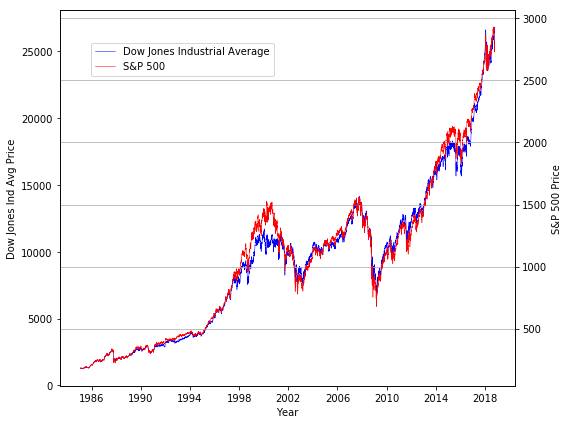
\includegraphics[width=0.8\linewidth]{time_series.png}
		\caption{Time series of Dow Jones and S\&P 500 indexes}
	\end{figure}
	
	\newpage
	%\pagebreak
	\subsection*{1.4 \& 1.5 \quad Chart of daily log returns from 30th January 1985 to 17th October 2018}
	
	\begin{figure}[h!]
		\centering
		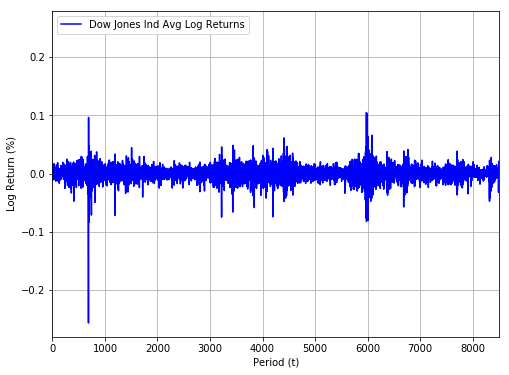
\includegraphics[width=0.8\linewidth]{DJI_logret.png}
		\caption{Time series of Dow Jones Index log returns}
	\end{figure}
	\begin{figure}[h!]
		\centering
		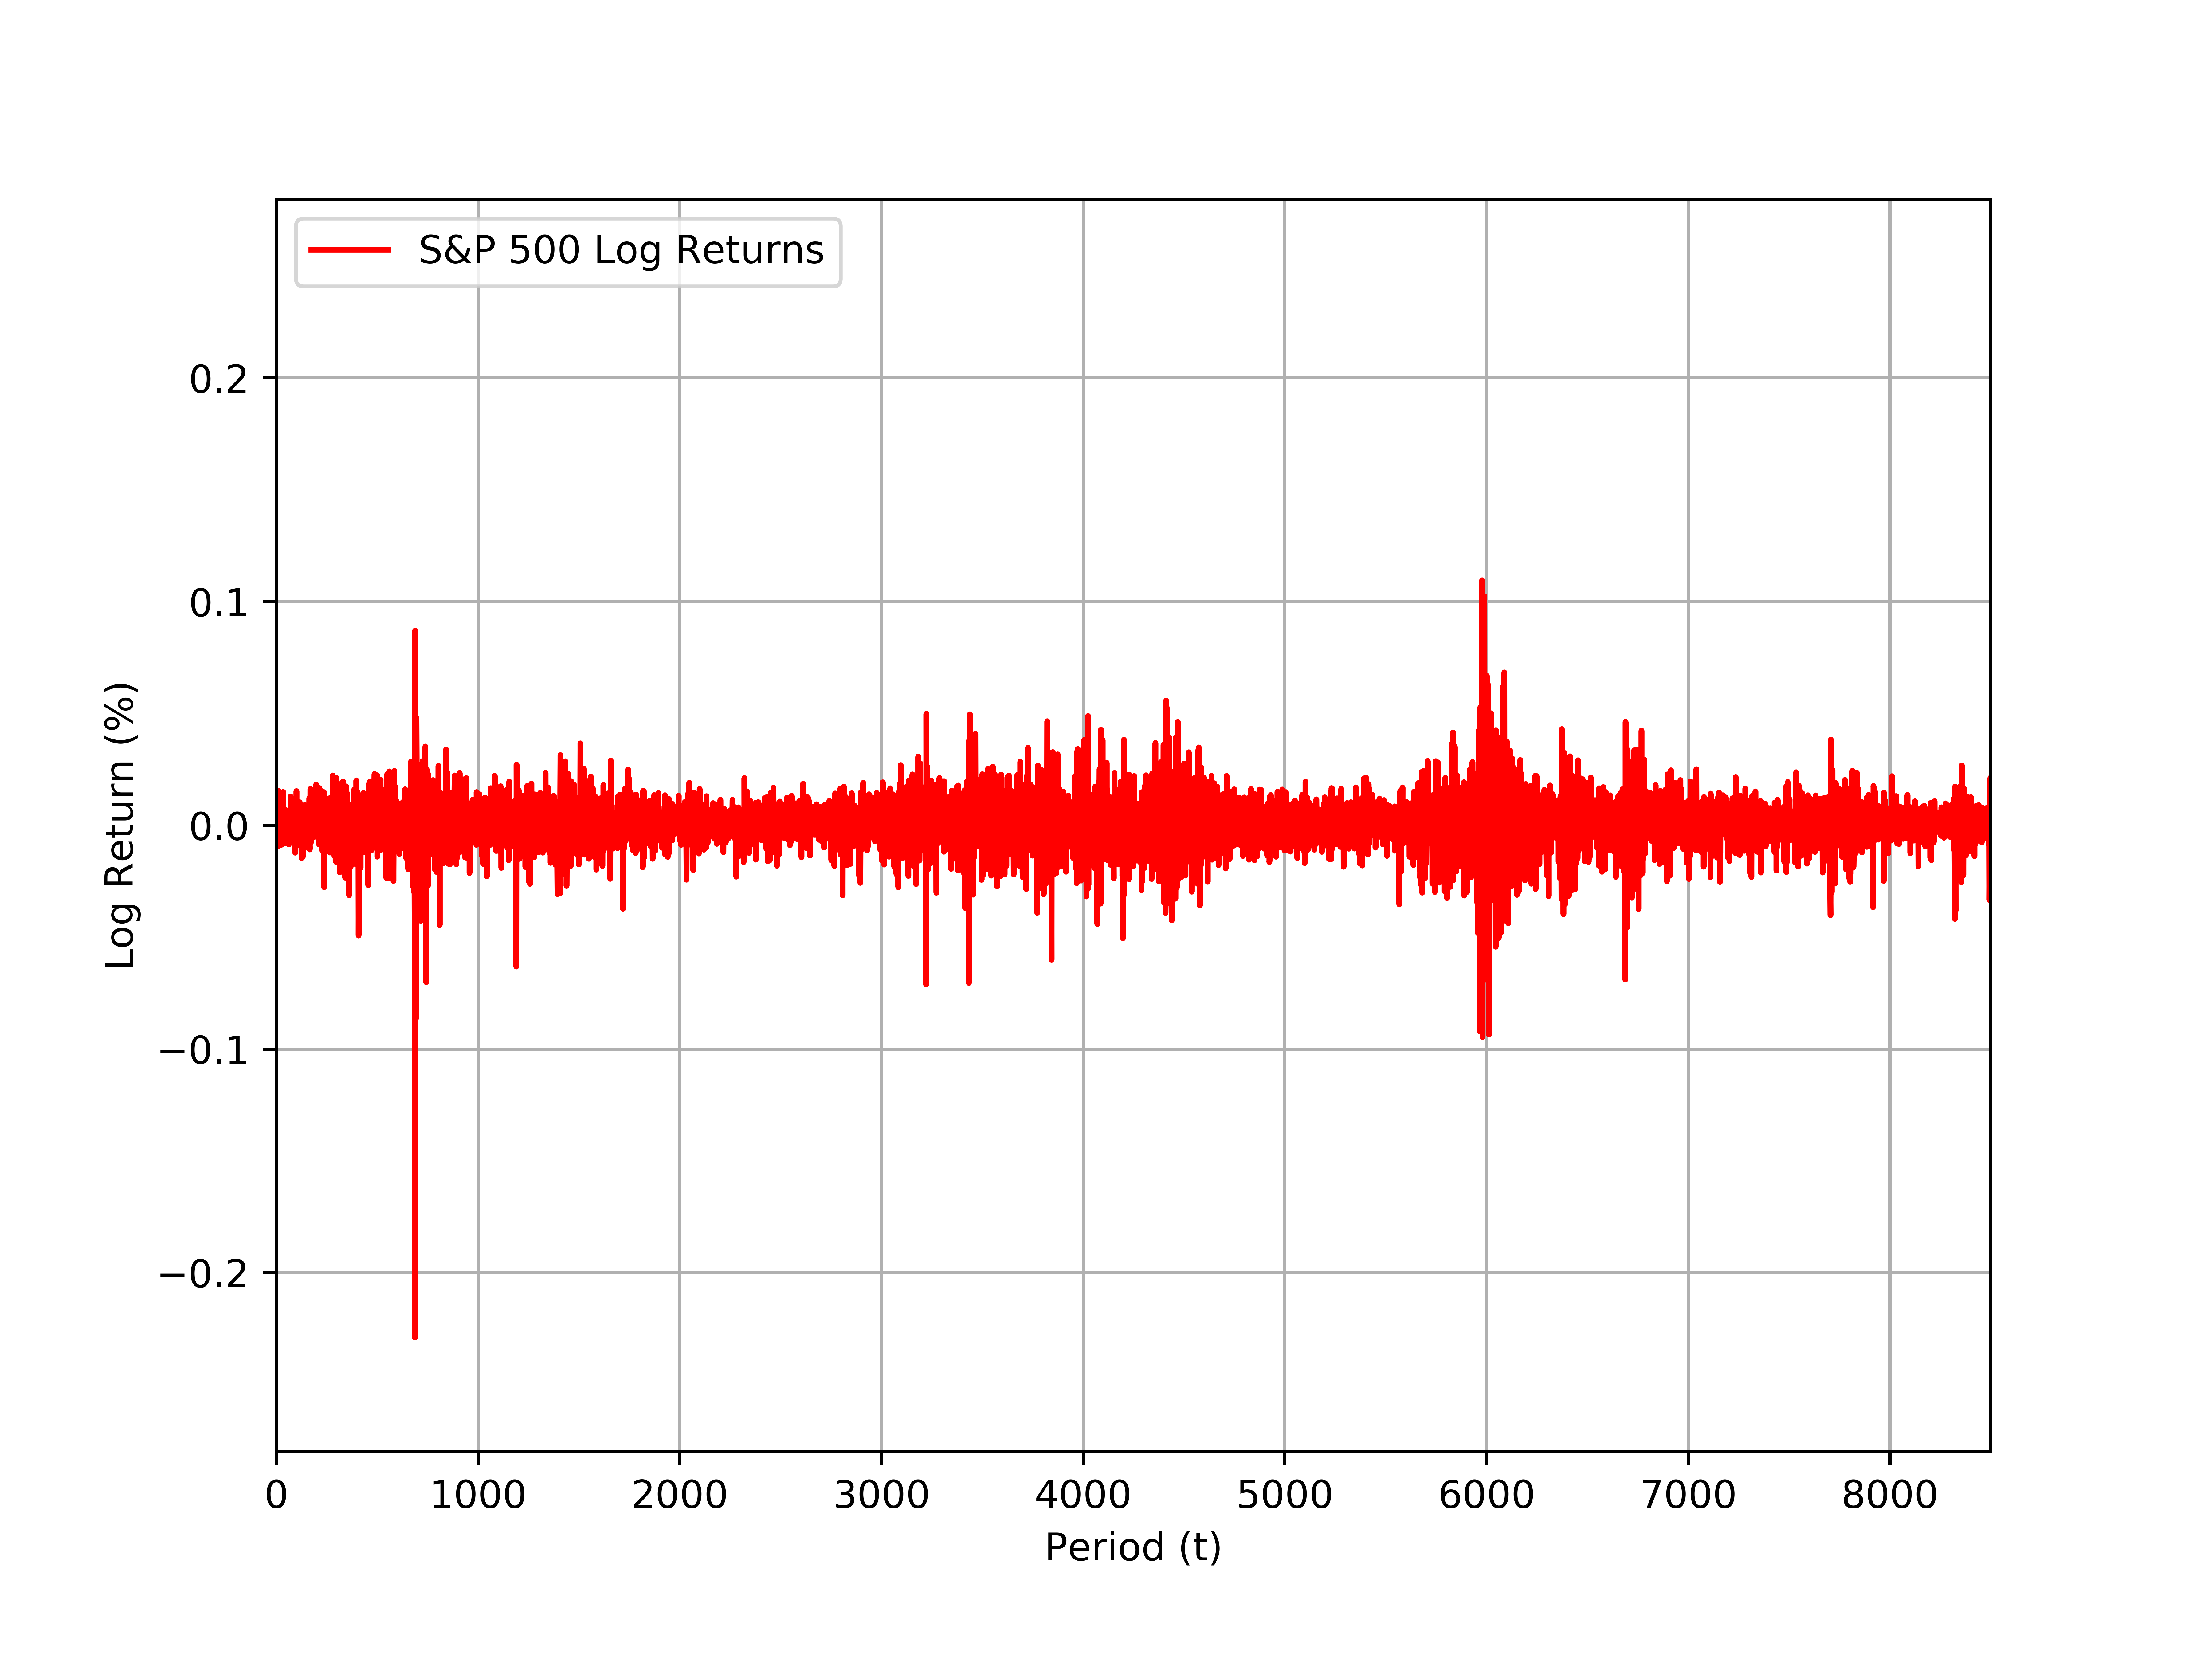
\includegraphics[width=0.8\linewidth]{SP_logret.png}
		\caption{Time series of S\&P 500 log returns}
	\end{figure}
	
	\setcounter{subsection}{5}
	\subsection{Sample mean and sample variance of log return}
	
	\begin{flushleft}
		Sample mean of Dow Jones Index : 0.0352\%  \linebreak 
		Sample mean of S\&P 500 Index : 0.0324\%  \linebreak 
		Sample variance of Dow Jones Index : $0.0121\%^2$  \linebreak 
		Sample variance of S\&P 500 Index : $0.0127\%^2$ \linebreak 
	\end{flushleft}
	
	\subsection{Annualized average and volatility of log return}
	\begin{flushleft}
		Annualized log return of Dow Jones Index : 8.8647\% \linebreak 
		Annualized volatility of Dow Jones Index : 17.4493\% \linebreak 
		Annualized log return of S\&P 500 Index : 8.1597\% \linebreak 
		Annualized volatility of S\&P 500 Index : 17.8570\% \linebreak 
	\end{flushleft}
	\vspace{-7mm}
	We use the additive feature of log returns to compute the annualized log return of Dow Jones and S\&P index. 
	
	We recognize that the S\&P index has a superior breadth and depth of coverage compared to the Dow. Therefore, we conclude firstly, that the annualized log return of US stock market is approximately equal to the S\&P’s (at 8.16\%).
	
	The annualized log returns of the Dow is about 0.7050\% higher than the S\&P’s. In contrast, the Dow’s volatility is 0.4077\% less than the S\&P’s. From this, we can draw 2 conclusions. Firstly, the Dow has a comparatively better Sharpe ratio, and therefore, has a better risk-reward profile. Secondly, the Dow is empirically less risky compared to the S\&P index. This in turn means that the Dow would have a lower Beta compared to overall US stock market.
	
	
	\subsection{Sample skewness and sample kurtosis}
	\begin{flushleft}
		Skewness of Dow Jones Index : -1.6916 \linebreak
		Kurtosis of Dow Jones Index : 45.3947 \linebreak
		Skewness of S\&P 500 : -1.2832 \linebreak
		Kurtosis of S\&P 500 : 31.4436 \linebreak
	\end{flushleft}
	\vspace{-7mm}
	The Dow and S\&P indices both have negative skewness, which means that the distribution of log returns is asymmetric and is left-skewed. There are several conclusions we can draw from this finding. Firstly, we know that a left-skewed distribution has a “drawn out” left tail – meaning, it has a longer and fatter left-tail. Also, we know that the mean of the distribution is smaller than the median, which itself is smaller than the mode. And, Finally, we know that the median is closer to the third quartile that to the first quartile. 
	
	Intuitively, we do not find that it is unusual to expect negative skewness in index returns because we observe more extreme downward movement (i.e. larger negative returns) during periods of recession.
	
	The Dow and S\&P have kurtosis values of 45.3947 and 31.4436 respectively. This is very high, considering that the kurtosis of a normal distribution is 3.0. Kurtosis is a measure of the sharpness of the peak of a frequency-distribution curve, and distributions with kurtosis greater than 3 are said to be leptokurtic. The high kurtosis of the Dow and S\&P indices' log return distributions, and by extension the US stock market return histogram, imply that the tails of the distributions approaches 0 more slowly than a normal distribution, and therefore produces more outliers than the normal distribution. 
	
	The implication of this finding is that extreme “events” like stock price crash or booms, which produce abnormally large returns (both positive and negative), are happening more often than what is predicted by the normal distribution.
	
	
	\subsection{Jarque-Bera test statistics}
	\begin{flushleft}
		Jarque-Beta Statistic of Dow Jones Ind Avg's Returns: 633852.49\linebreak
		Jarque-Beta Statistic of S\&P's Returns: 285696.06\linebreak
		Critical Chi-Square Value with 2 Degrees of Freedom: 5.991465\linebreak
	\end{flushleft}
	\vspace{-7mm}
	The JB test’s null hypothesis is JB = 0. If the null hypothesis is not rejected, it indicates that the distribution that we are testing has a normal distribution (under a certain level of significance).  
	
	The critical Chi-Square Value with 2 Degrees of Freedom and a 5\% significance level is 5.9915. The JB test statistic for both the Dow and S\&P are above that critical value. We therefore reject the null hypothesis for both the S\&P as well as the Dow. And, we conclude that based on the JB test at the 5\% significance level, the log return of these two indices are not normally distributed.
	
	We plotted the frequency-distribution histogram, overlaid with a normal distribution curve with the same mean and variance as the underlying data. From the image, we noted the histogram for both the S\&P and DJI have sharper peaks and fatter tails. This indicates that the distributions of log returns for both indices are not normally distributed as they have "significant excess kurtosis".
	
	Furthermore, as seen from the range of the histogram plot (x-axis), there are a number of extreme "high sigma" events. The normal distribution predicts that these events will occur with close to zero probability, therefore, the very existence of such events indicate the underlying data is not normally distributed. 

	\newpage	
	\begin{figure}[h!]
		\centering
		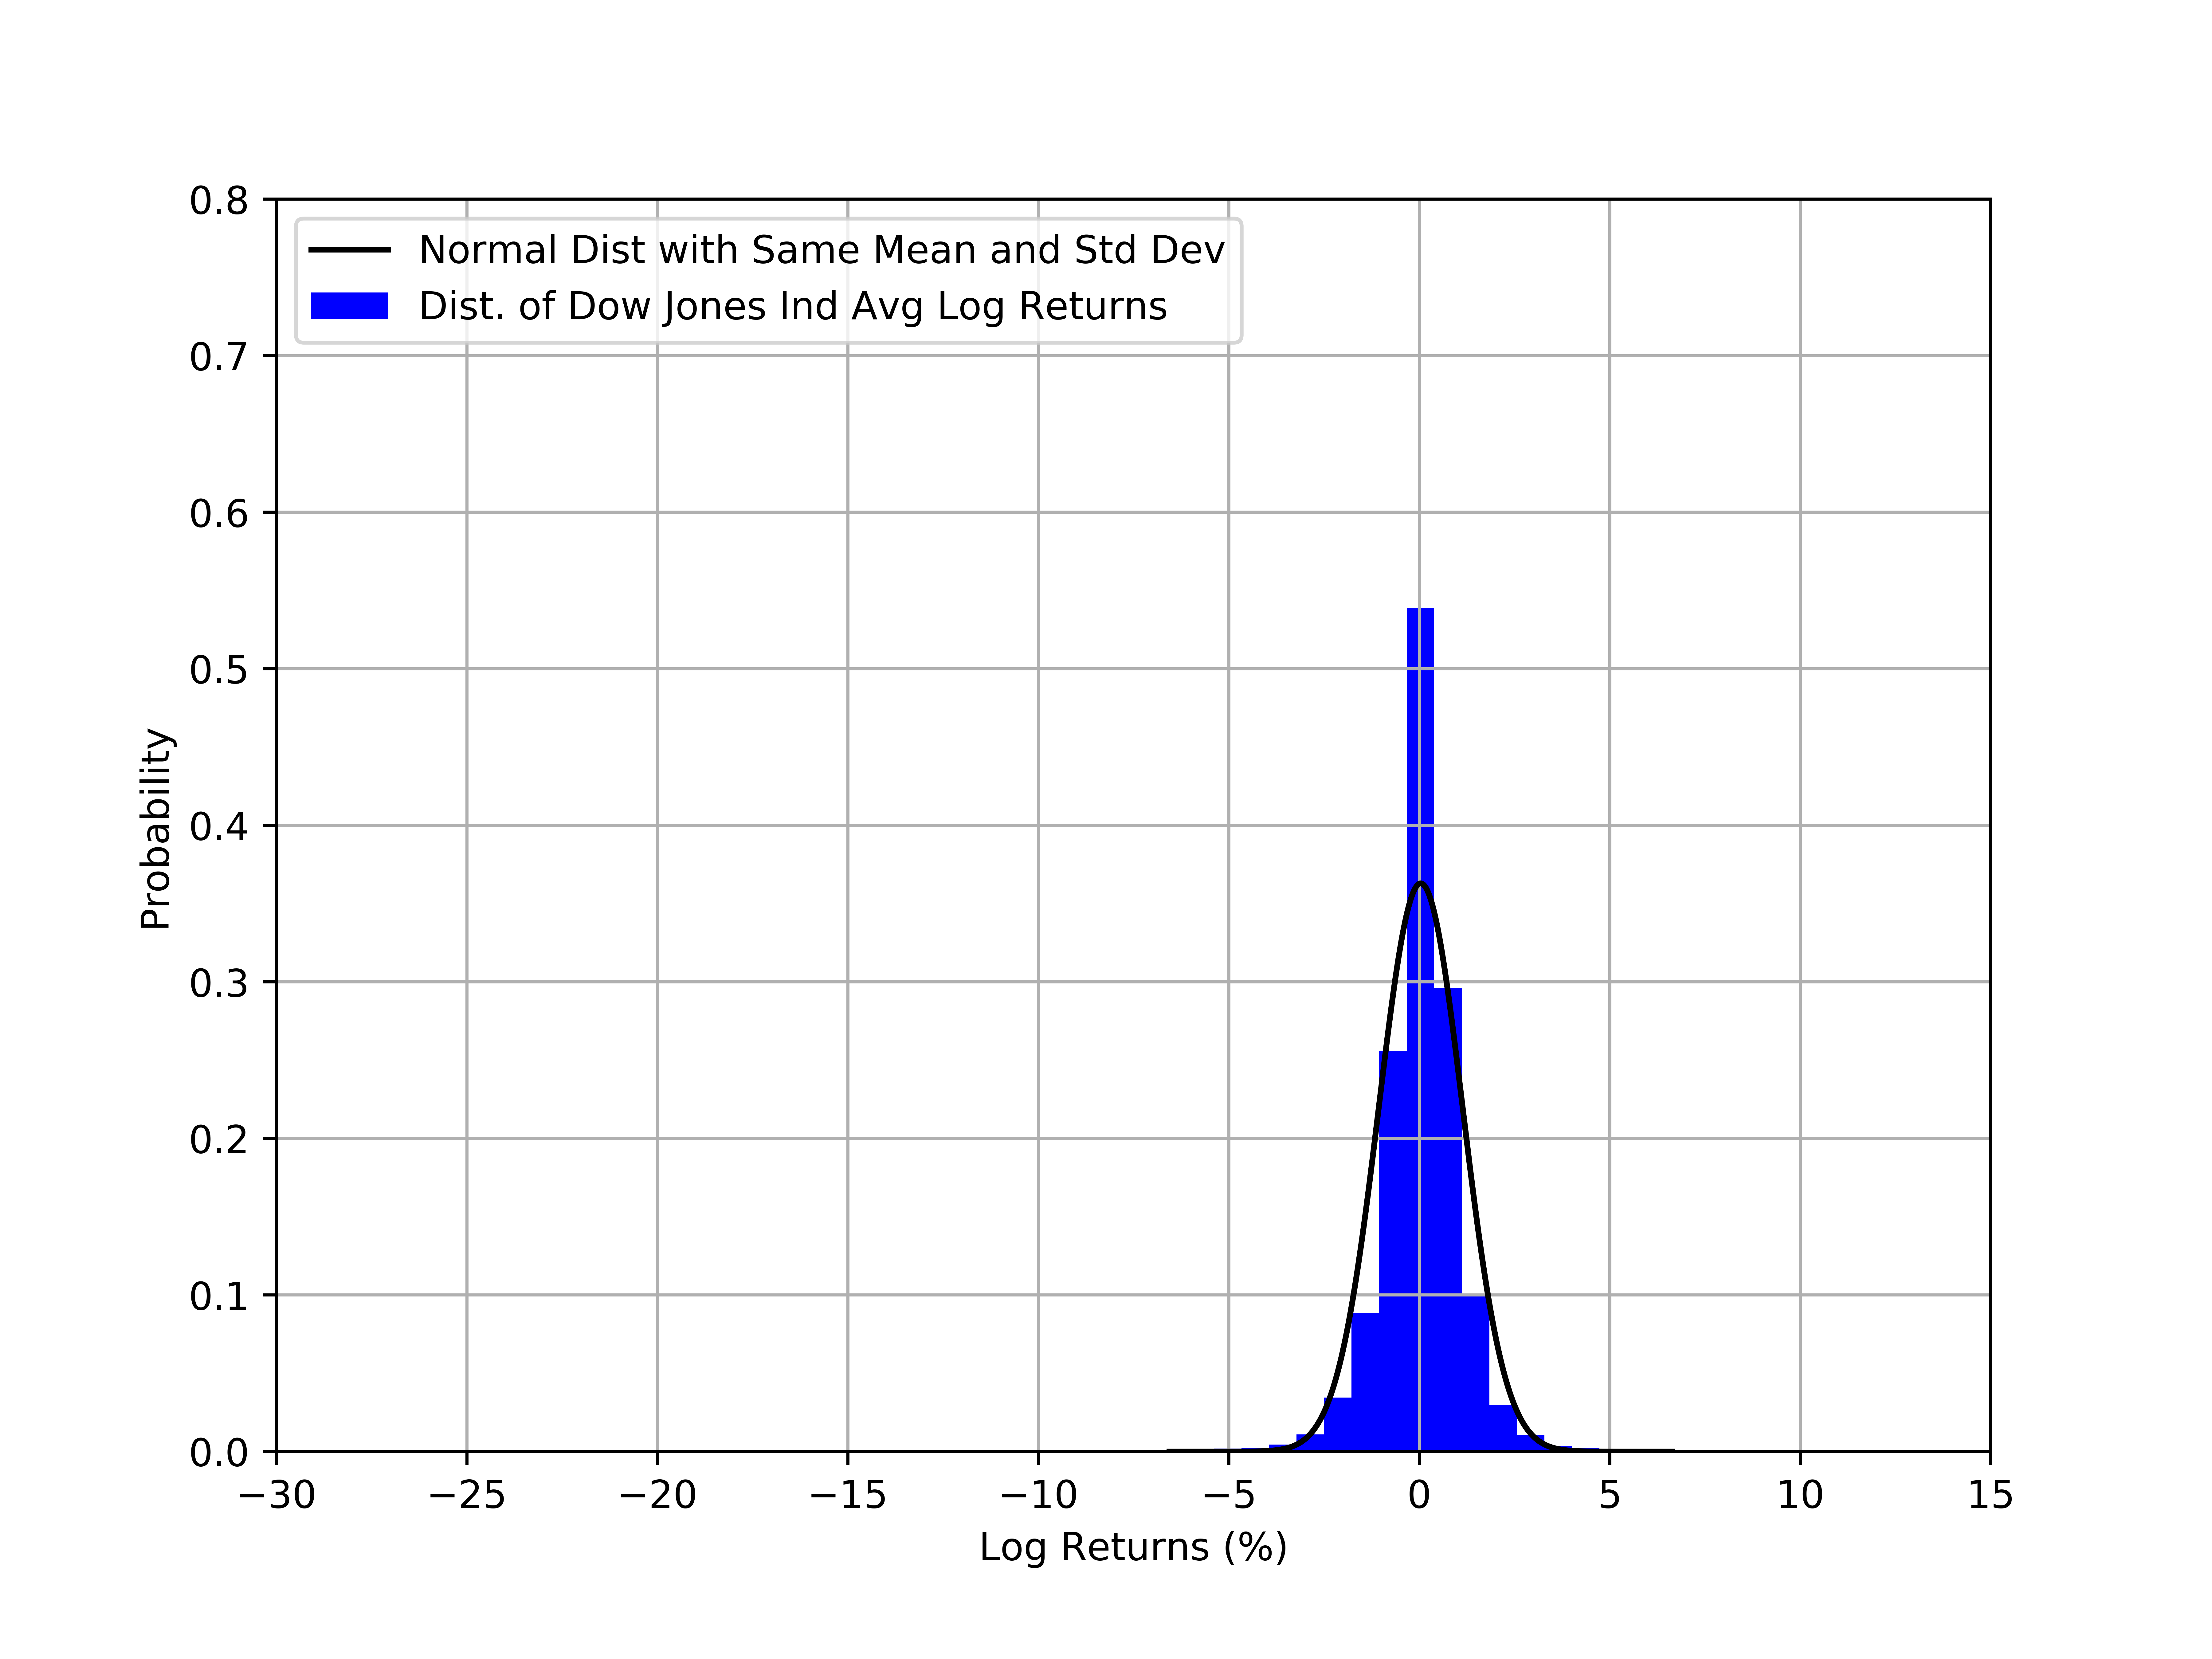
\includegraphics[width=0.8\linewidth]{DJInorm.png}
		\caption{Distribution of Dow Jones Index log returns from 30th January 1985 to 17th October 2018}
	\end{figure}
	\begin{figure}[h!]
		\centering
		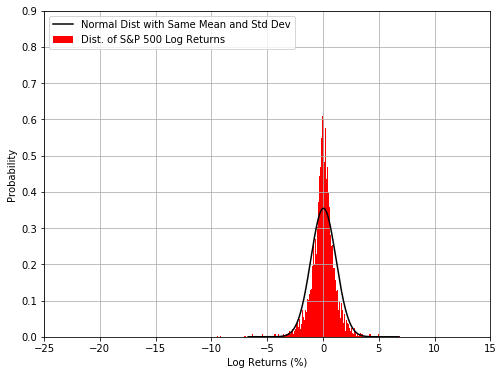
\includegraphics[width=0.8\linewidth]{GSPCnorm.png}
		\caption{Distribution of S\&P 500 log returns between from 30th January 1985 to 17th October 2018}
	\end{figure}
	
	\newpage
	\section{Task2}
	\label{sec:introduction}
	
	\subsection{Correlation between log returns of the Dow Jones Index and S\&P 500}
	The correlation of the daily log returns from 30th January 1985 to 17th October 2018 is 0.9651. As the correlation is very close to 1, we say that the daily log returns of the S\&P and Dow are highly correlated. We believe that the high correlation can be explained by the fact that the Dow’s 30 component stocks are also included in the S\&P index. 
	
	When we analyse the correlation on a 252-day rolling basis, we noted that there are periods where the correlation drops sharply to approximately 0.8. This finding is logical because the Dow, unlike the S\&P, is sometimes affected by large price swings in one of its component stocks. The same price swing would not affect the S\&P as much because of the S\&P’s broader coverage. 
	
	\begin{figure}[h!]
		\centering
		\includegraphics[width=0.8\linewidth]{correlation.png}
		\caption{Correlation between log returns of the Dow Jones Index and S\&P 500 from 30th January 1985 to 17th October 2018}
	\end{figure}
	
	\newpage
	\subsection{Two-sample t-test of the two indexes}
	\begin{flushleft}
		t Statistic: 0.164005
		
		Critical t Values: +/-1.960104
		
		Thus, we are unable to reject null hypothesis that mean differences are 0.
	\end{flushleft}
	
	\subsection{F-test of the two indexes}
	\begin{flushleft}
		F Statistic: 1.047283
		
		Critical F Values: 0.958368, 1.04344
		
		Thus, we are able to reject null hypothesis that the 2 population variances are equal.
	\end{flushleft}
	
	%\newpage
	%\begin{thebibliography}{9}
	%\bibitem{nano3}
	%  K. Grove-Rasmussen og Jesper Nygård,
	%  \emph{Kvantefænomener i Nanosystemer}.
	%  Niels Bohr Institute \& Nano-Science Center, Københavns Universitet
	
	%\end{thebibliography
\end{document}
